
\section{\lsystem types}
\label{sec:lsysTypes}

In this section is described different types of \lsystems.
Some types may require an extension to the described formal definition of an \lsystem but this will be omitted here.

The \lsystems described so far are called \emph{deterministic \lsystems} because their rewriting system is deterministic.
\emph{Bracketed \lsystems} allow to save and load a state of the interpretation;
	this can be used to model branches of plants more easily.
\emph{Stochastic \lsystems} can randomize a result model to suppress its artificiality.
\emph{Context-sensitive \lsystems} allow to rewrite symbols depending on their context (the neighboring symbols around them).
Symbols in \emph{parametric \lsystems} can hold any number of arguments that can be used while rewriting or interpreting symbols.

Any of the above-described types can be combined together.



\subsection{Deterministic \lsystems}

\newcommand{\dzerolsystem}{\mbox{D0L-system}\xspace}
\newcommand{\dlsystem}{\mbox{dL-system}\xspace}


\begin{wrapfigure}{r}{0.50\textwidth}
	\vspace{-30pt}
	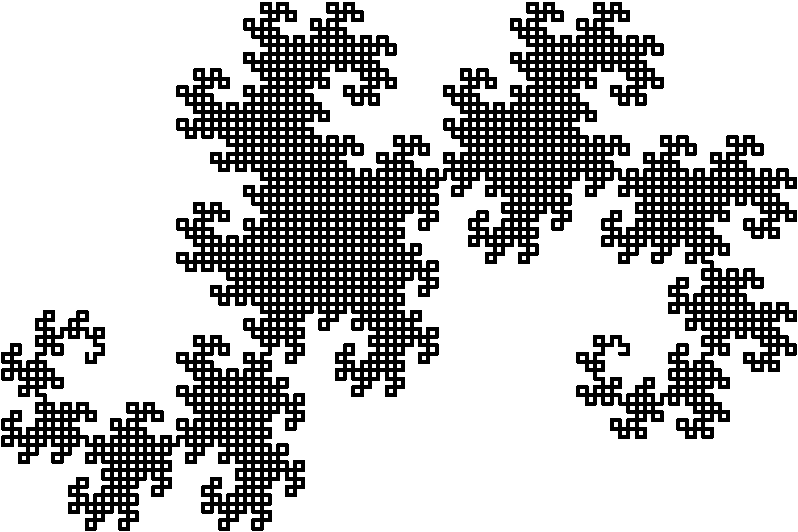
\includegraphics[width=\linewidth]{BasicLsystem}
	\caption{Dragon curve}
	\label{fig:basicLsystem}
\end{wrapfigure}


The basic \lsystem type described by the previous formal definition is called a \dzerolsystem\footnote{A \dzerolsystem is also just called a \dlsystem~\cite{Zar04}.}.
\emph{D} means that the rewriting is deterministic and \emph{0} means it is context-free.
The result of a \dzerolsystem depends only on the initial string of symbols.

This type of \lsystem is often used to generate fractal curves.
With the \dzerolsystem in \autoref{fig:basicLsystem} we can generate the Dragon curve that you can see in \autoref{lsys:basicLsystemSrc}.

\begin{Lsystem}[label=lsys:basicLsystemSrc,caption={\dzerolsystem for the generation of the Dragon curve (\autoref{fig:basicLsystem})}]
lsystem DragonCurve {
	set iterations = 12;
	set symbols axiom = L;
	interpret R L as DrawForward(5);
	interpret + as TurnLeft(90);
	interpret - as TurnLeft(-90);
	rewrite L to L + R +;
	rewrite R to - L - R;
}
process all with SvgRenderer;
\end{Lsystem}


\subsection{Bracketed \lsystems}

A bracketed \lsystems\cite[p.~24]{PL91} extends basic \dzerolsystem with a branching system.
Branching is such a fundamental feature that Bracketed \lsystems are often just called \lsystems.

A branching system brings two new commands to the symbol interpretation system: \emph{start branch} and \emph{end branch}.
These commands are nearly always represented as bracket symbols (from which bracketed \lsystems got their name).
An open bracket "\texttt{[}" as a start branch and close bracket "\texttt{]}" as a close branch.

The start branch command saves the state of interpretation, which can then be loaded by end the branch command later.
In turtle graphics, the interpretation state is the position, orientation and drawing color of the turtle.
More than one state can be saved at the same time, and the last saved state will be loaded first.
This behavior seems natural and could be compared to a pairing of brackets.

Branching extends a linear string of symbols to a tree structure.
Individual branches do not affect each other nor their root.
This allows plants to be modeled more easily and to create more complex models.

The bracketed \lsystem in \autoref{lsys:branchingSrc} demonstrates a use of the branching system to produce a plant-like model as can be seen in \autoref{fig:branching}.
Note that the color of segments indicates their type and age.
Black segments are drawn with the symbol \texttt{F} and they represent segments from the previous iteration.
Green segments are drawn with the symbol \texttt{A} and they are new compared to the previous iteration.

\begin{Lsystem}[label=lsys:branchingSrc,caption={A bracketed \lsystem that which creates a plant-like model (\autoref{fig:branching})}]
lsystem PythagorasTree {
	set symbols axiom = A;
	set initialAngle = 90;
	set iterations = 4;	
	interpret A F as DrawForward(16);
	interpret + as TurnLeft(45);
	interpret - as TurnLeft(-45);
	@interpret [ as StartBranch;@
	@interpret ] as EndBranch;@
	rewrite A to F [ + A ] [ - A ] F A;
	rewrite F to F F;
}
process all with SvgRenderer;
\end{Lsystem}

\begin{figure}[h]
	\centering
	\subfloat{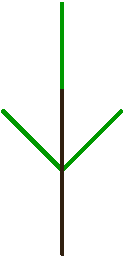
\includegraphics[scale=1]{Branching1}} ~
	\subfloat{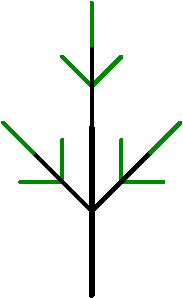
\includegraphics[scale=1]{Branching2}} ~
	\subfloat{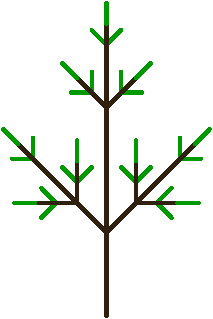
\includegraphics[scale=1]{Branching3}} ~
	\subfloat{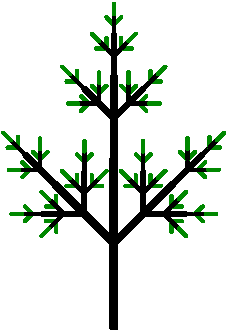
\includegraphics[scale=1]{Branching4}}
	\caption[The first four iterations of a bracketed \lsystem]{The first four iterations of the bracketed \lsystem in \autoref{lsys:branchingSrc}}
	\label{fig:branching}
\end{figure}



\subsection{Stochastic \lsystems}

\newcommand{\zerolsystem}{\mbox{0L-system}\xspace}
\newcommand{\zerolsystems}{\mbox{0L-systems}\xspace}

All plant models generated by the same deterministic \lsystem are identical.
However, a forest made by trees which are all identical looks artificial and can not be used in films or video games.
Stochastic \lsystems solve this problem because they can produce a randomized model.
Stochastic \lsystems are called \zerolsystem where 0 means they are context-free.

Randomization of a model produced by stochastic a \lsystem can be done in two places, in the rewrite rules or in the interpretation of symbols (or in both).
Randomization in interpretation can only change the properties of such interpreted symbols as lengths of lines or turning angles, while the topology of the model remains unchanged.
This is in contrast to rewrite rule randomization that can also change the topology of a model.
Rewrite rule randomization is achieved by defining more replacements for one rewrite rule.
The rewriting system will pick a random replacement if the rewrite rule is applied.
Each replacement can have a different probability of being picked.

In \autoref{fig:randComparison}, three models of a plant generated by stochastic \lsystems are shown.
The first image (\ref{fig:randComparisonNo}) was generated without any randomization.
The second image (\ref{fig:randComparisonInt}) was generated with interpretation randomization of line lengths and angles.
For the last image (\ref{fig:randComparisonBoth}) was used the rewrite rule randomization which changed the topology of the model (\autoref{lsys:randExample}).

\begin{figure}[h]
	\centering
	\subfloat[No randomization]{
		\label{fig:randComparisonNo}
		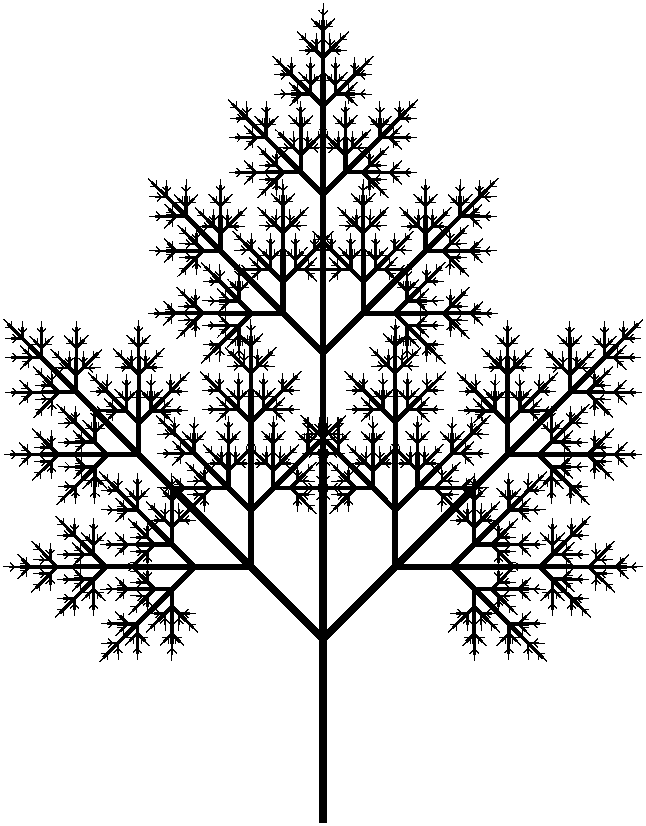
\includegraphics[width=0.3\textwidth]{StochasticLsystemExample-NoStochasism}
	} ~
	\subfloat[Angles, lengths randomized]{
		\label{fig:randComparisonInt}
		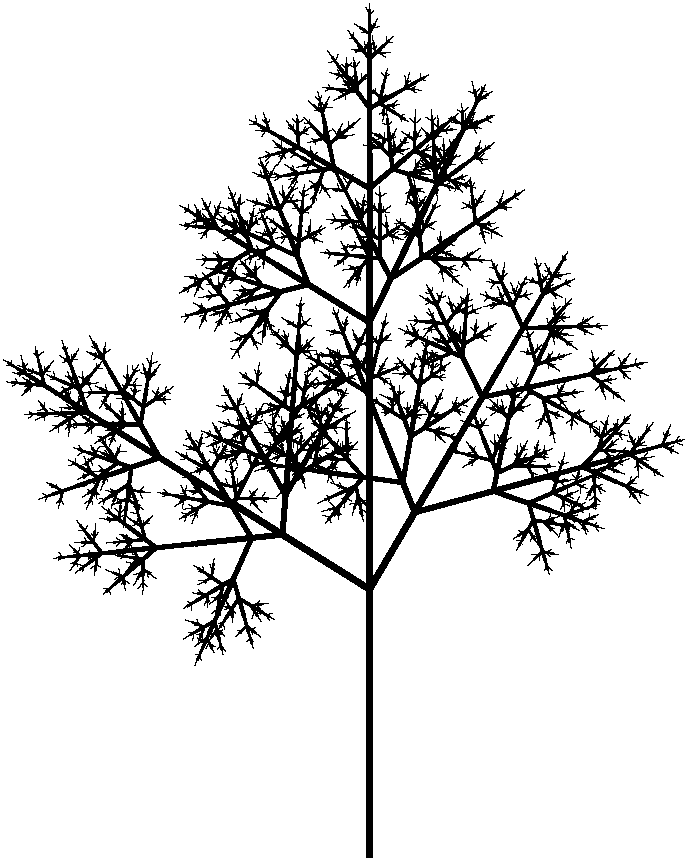
\includegraphics[width=0.32\textwidth]{StochasticLsystemExample-InterpretationStochasism}
	} ~
	\subfloat[Also topology randomized]{
		~
		\label{fig:randComparisonBoth}
		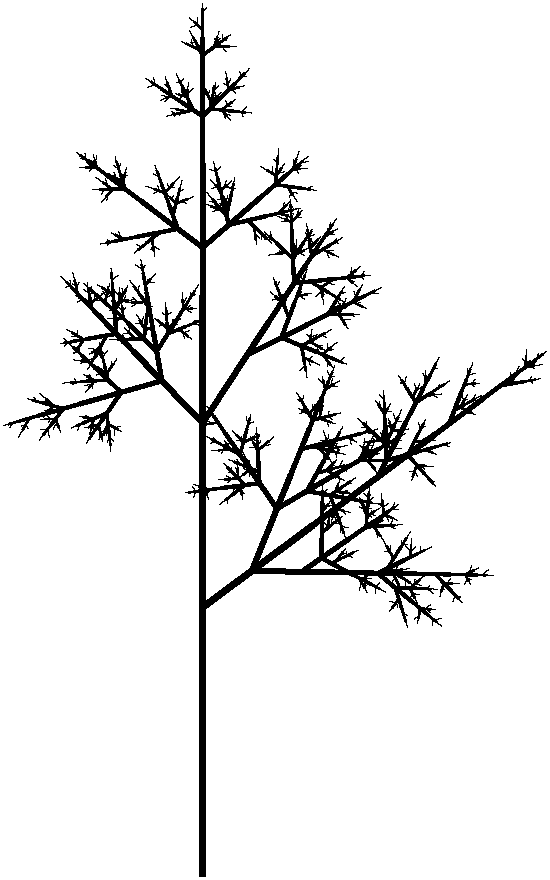
\includegraphics[width=0.25\textwidth]{StochasticLsystemExample-BothStochasism}
		~
	}
	\caption{A comparison between a non-randomized and randomized plant model}
	\label{fig:randComparison}
\end{figure}

\begin{Lsystem}[label=lsys:randExample,caption={Stochastic \lsystem with randomized interpretation of symbols and rewrite rule replacements}]
lsystem StochasticLsystemExample {
	set symbols axiom = X;
	set iterations = 8;
	set initialAngle = 90;
	interpret F(age) as DrawForward(@1.8^age*random(0.5,1.5)@, age/2);
	interpret + as TurnLeft(@45 + random(-20, 20)@);
	interpret - as TurnLeft(@-45 + random(-20, 20)@);
	interpret [ as StartBranch;
	interpret ] as EndBranch;
	rewrite F(age) to F(age + 1);
	@rewrite X@
		@to F(1) [ + X ] [ - X ] F(1) X  weight 4 or@
		@to F(1) [ + X ]         F(1) X  weight 1 or@
		@to F(1)         [ - X ] F(1) X  weight 1;@
}
process all with SvgRenderer;
\end{Lsystem}


\subsection{Context-sensitive \lsystems}

\newcommand{\onelsystems}{\mbox{1L-systems}\xspace}
\newcommand{\twolsystems}{\mbox{2L-systems}\xspace}

The rewriting of symbols in \zerolsystems is context-free; the rewrite rules are applied to the symbols regardless of their context (the symbols around them).
However, the rewriting of a symbol can also depend on its context.
This is useful in simulating the flow of signals (nutrients or hormones) in a plant model that, for example, attempts to demonstrate natural plant growth~\citep{PL91}.

Formally there are two types of context-sensitive L-systems, \onelsystems and \twolsystems.
The rewrite rules of \onelsystems checks the context only to one side (left or right), whereas the rewrite rules of \twolsystems checks the context on both sides.
Since \onelsystems are just \twolsystems with one context empty we will consider context-sensitive \lsystems as \twolsystems.

The context-sensitive \lsystem in \autoref{lsys:signalPropagarionSrc} shows a simulation of signal propagation in a string of symbols; the result is given in \autoref{fig:signalPropagarion}.

\begin{Lsystem}[label=lsys:signalPropagarionSrc,caption={Context-sensitive \lsystem simulating signal propagation}]
lsystem RewritingExample {
	set symbols axiom = B A A A A A;
	set iterations = 6;
	set interpretEveryIteration = true;
	@rewrite {B} A     to B;@
	@rewrite     B {A} to A;@
}
process all with SymbolPrinter;
\end{Lsystem}

\begin{table}[h]
	\centering
	\begin{tabular}{c l}
   		\toprule
   		Iteration & String of symbols \\
   		\midrule
		0 & B A A A A A \\
		1 & A B A A A A \\
		2 & A A B A A A \\
		3 & A A A B A A \\
		4 & A A A A B A \\
		5 & A A A A A B \\
		6 & A A A A A A \\
		\bottomrule
	\end{tabular}
	\caption{An axiom and the first 6 iterations of an \lsystem in \autoref{lsys:signalPropagarionSrc} showing signal propagation in the given string of symbols}
	\label{fig:signalPropagarion}
\end{table}


\subsubsection{Context-sensitive bracketed \lsystems}
\label{sec:bracketedLsystems}

If we add context-sensitive rewrite rules to bracketed \lsystems the situation becomes more difficult.
The context-matching procedure must take into account the branches.
The following rules define the natural behavior of context between branches:
\begin{enumerate*}
	\item \label{enum:ctxRule1} two symbols are neighbors even if there are some branches between them,
	\item \label{enum:ctxRule2} the left neighbor of the first symbol in a branch is a symbol before the branch,
	\item \label{enum:ctxRule3} the last symbol in a branch does not have a right neighbor,
	\item \label{enum:ctxRule4} unmatched symbols at the end of a branch are ignored,
	\item \label{enum:ctxRule5} the order of branches is insignificant.
\end{enumerate*}

In \autoref{tbl:bracketCtxt} is a few examples of how a symbol with its context will match (or not) a given string of symbols with respect to the context-matching rules mentioned above.
\begin{table}[h]
	\centering
	\begin{tabular}{c c c | p{128pt} c c}
   		\toprule
   		Left ctx. & Symbol & Right ctx. & Symbol string & Match & Rule\\
   		\midrule
		 & X & Y & A B {\btHL\bf X} [ A [ B ] ] [ C ] {\btHL\bf Y} & yes & \ref{enum:ctxRule1} \\
		 & X & Y & A B X [ Y B ] C Y & no &  \\
		 Y & X & & A B {\btHL\bf Y [ X} A B ] C & yes & \ref{enum:ctxRule2} \\
		 Y & X & & A B {\btHL\bf Y [ [ X} A ] B ] C & yes & \ref{enum:ctxRule2} \\
		 & X & Y & A [ B X ] Y & no & \ref{enum:ctxRule3} \\
		 & X & [ Y ] & A B {\btHL\bf X [ Y} A B ] A  & yes & \ref{enum:ctxRule4} \\
		 & X & [ [ Y ] ] & A B {\btHL\bf X [ [ Y} A B ] C ] & yes & \ref{enum:ctxRule4} \\
		 & X & [ Y ] & A B {\btHL\bf X} [ A B ] {\btHL\bf{}[ Y} ] A  & yes & \ref{enum:ctxRule5} \\
		 & X & [ Y ] [ Z ] & A B {\btHL\bf X [ Z} ] {\btHL\bf{}[ Y} ] A  & yes & \ref{enum:ctxRule5} \\
		\bottomrule
	\end{tabular}
	\caption{Examples of context matching in bracketed \lsystems}
	\label{tbl:bracketCtxt}
\end{table}

Context in bracketed \lsystems can be used for the propagation of signals through tree structures.
There are two basic types of signals: the first is the \emph{acropetal} signal which spreads from the root to branches; and the second signal is \emph{basipetal} which spreads in the opposite way i.e. from branches to root.
This can be very useful in plant modeling.

\autoref{fig:signalPropagation} shows a simulation of acropetal (\ref{fig:acropetalSignal}) and basipetal (\ref{fig:basipetalSignal}) signals in a static plant-like structure.
Each figure shows the first 5 iterations and segments with the signal marked as a bolder line.
The \lsystem in \autoref{lsys:signalPropagation} simulates acropetal signal propagation and its result is in \autoref{fig:acropetalSignal} (image) and \autoref{fig:signalPropagationTable} (symbols).

\begin{figure}[h!]
	\centering
	\subfloat[Acropetal signal propagation]{
		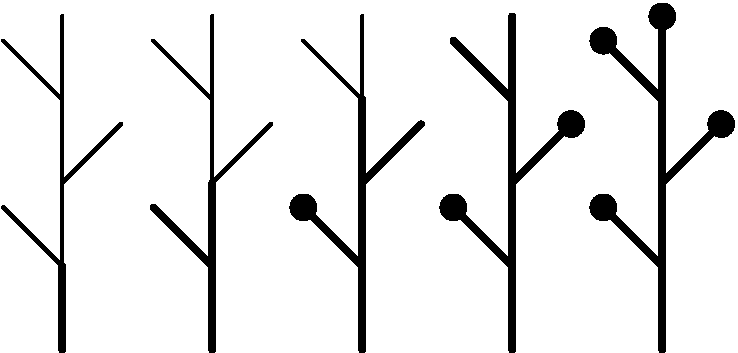
\includegraphics[scale=0.55]{AcropetalSignal}
		\label{fig:acropetalSignal}
	}
	\hspace{2mm}
	\subfloat[Basipetal signal propagation]{
		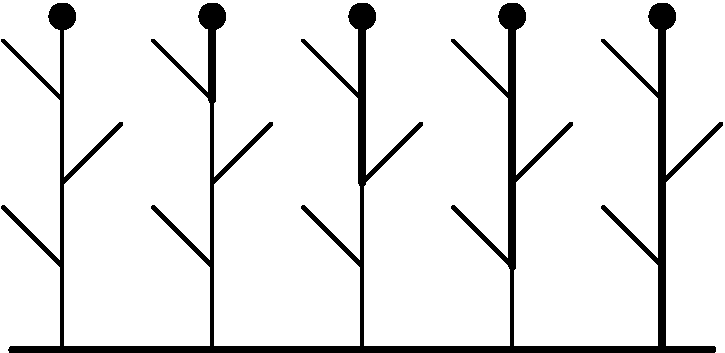
\includegraphics[scale=0.55]{BasipetalSignal}
		\label{fig:basipetalSignal}
	}
	\caption{Signal propagation simulated with context-sensitive bracketed \lsystems}
	\label{fig:signalPropagation}
\end{figure}

\begin{Lsystem}[label=lsys:signalPropagation,caption={The \lsystem simulating acropetal signal propagation (\autoref{fig:acropetalSignal})}]
lsystem AcropetalSignal extends Branches {
	set symbols axiom = B [ + A ] A [ - A ] A [ + A ] A;
	// ignore + and - symbols in context search
	@set symbols contextIgnore = + -;@
	set iterations = 3;
	// interpret every iteration to see signal propagation
	set interpretEveryIteration = true;
	set initialAngle = 90;
	interpret A as DrawForward(50, 2);
	interpret B as DrawForward(50, 4);
	interpret + as TurnLeft(45);
	interpret - as TurnLeft(-45);
	@rewrite { B } A to B;@
}
process all with SvgRenderer;
\end{Lsystem}


\begin{table}[h]
	\centering
	\begin{tabular}{c c}
   		\toprule
   		Iteration & String of symbols \\
   		\midrule
		0 & B [ + A ] A [ - A ] A [ + A ] A \\
		1 & B [ + B ] B [ - A ] A [ + A ] A \\
		2 & B [ + B ] B [ - B ] B [ + A ] A \\
		3 & B [ + B ] B [ - B ] B [ + B ] B \\
		\bottomrule
	\end{tabular}
	\caption{The result of the \lsystem simulating acropetal signal propagation in \autoref{lsys:signalPropagation}}
	\label{fig:signalPropagationTable}
\end{table}


\subsection{Parametric \lsystems}

Symbols in parametric \lsystems can hold any number of arguments.
Arguments are often floating point numbers, but they can be much more complicated structures.
Arguments can be used in interpretation definition to send values like color or length of line to an interpretation routine.
Arguments can also be used in rewrite rules to determine whether to rewrite a symbol or not, and to determine new arguments for rewritten symbols.
In context \twolsystems it is also possible to get arguments from symbols in context and use them in rewrite rules.

The \lsystem in \autoref{fig:scParams} shows an example of how the parameters of symbols can be used in interpretation methods and in rewrite rules together with the result.

\newsavebox{\lstBox}
\begin{lrbox}{\lstBox}
\begin{Lsystem50}
lsystem Circles {
	set symbols axiom =	[ X ] +
		[ X ] + [ X ] + [ X ];
	set iterations = 7;
	interpret F as MoveForward;
	interpret K as DrawCircle;
	interpret + as @TurnLeft(90)@;
	interpret - as @TurnLeft(-90)@;
	interpret [ as StartBranch;
	interpret ] as EndBranch;
	rewrite @K(n) to K(2*n)@;
	rewrite @F(n) to F(2*n)@;
	rewrite X to @K(2) F(3)@
		[ + X ] [ - X ] X;
}
process all with SvgRenderer;
\end{Lsystem50}
\end{lrbox}

\begin{figure}[h!]
	\subfloat{
		\usebox{\lstBox}
	} \hfill
	\subfloat{
		\minipage{0.47\linewidth}\noindent
		
\includegraphics[width=\textwidth]{Circles}
		\endminipage
	}
	\caption{Parameters usage in \lsystem interpretation methods and in rewrite rules along with the result}
	\label{fig:scParams}
\end{figure}

In \autoref{fig:redEndPythagoras} is more complicated model, the Pythagoras tree.
Detailed instructions for its construction with \lsystems are described in appendix \ref{chap:userDoc}.

\begin{figure}[H]
	\centering
	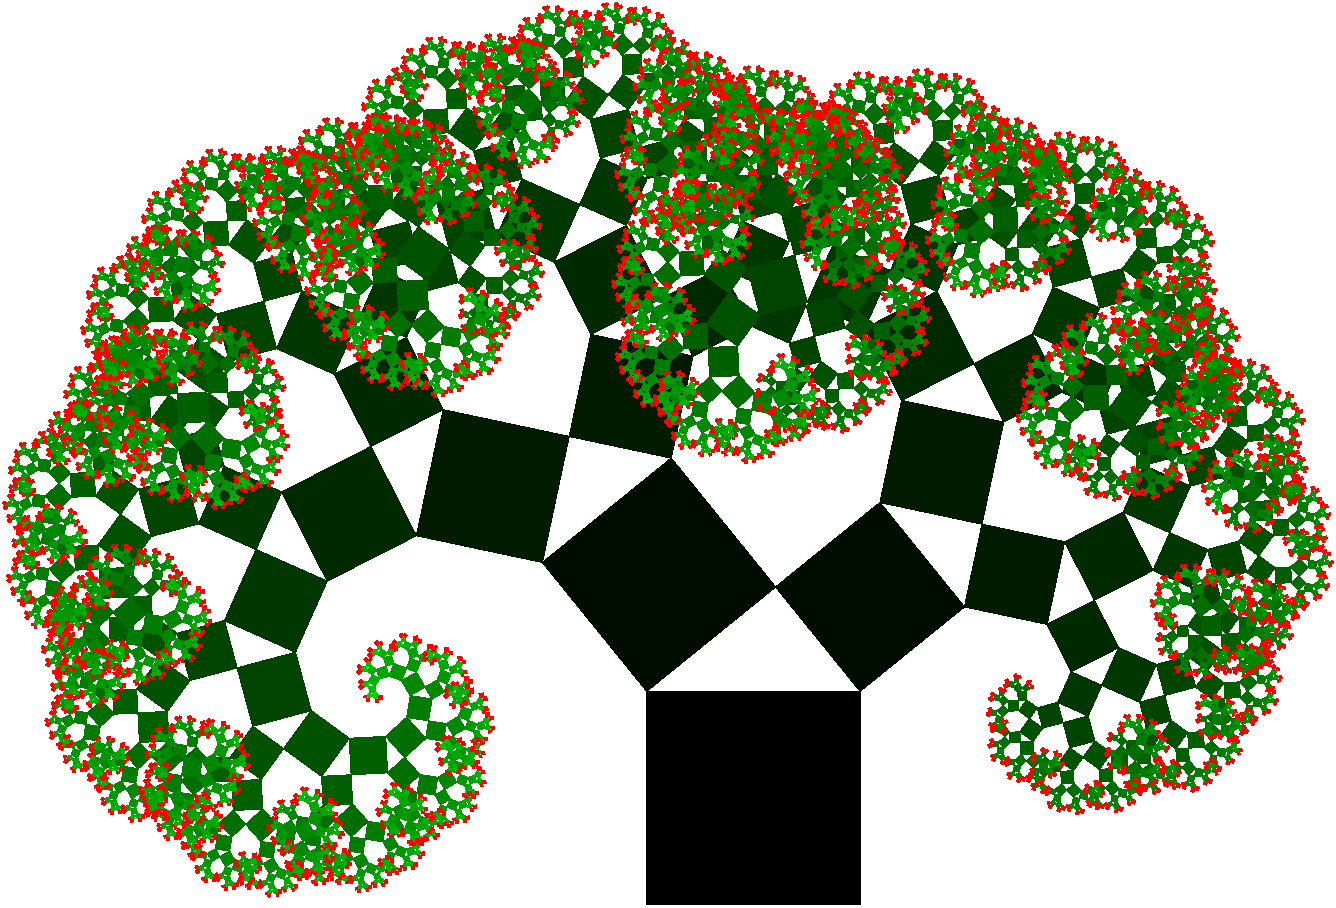
\includegraphics[width=\linewidth]{PythagorasTree2dRedEnd}
	\caption{Pythagoras tree created with parametric \lsystem}
	\label{fig:redEndPythagoras}
\end{figure}
































